\documentclass[conference,9pt]{IEEEtran}
\usepackage{xcolor}
\usepackage{cite}
\usepackage{epsfig}
\usepackage{amssymb}
\usepackage{amsmath}
\usepackage{graphicx}
\graphicspath{ {./} }

\begin{document}
\title{Practical 2a}

\author{
\IEEEauthorblockN{Albert Acebron}
\IEEEauthorblockA{NIU: 1458626}
}


% make the title area
\maketitle
\begin{abstract}
This practical will be based on applying ML to received signals to estimate their phase
\end{abstract}



%----------------------------------------------------------------
% SECTION #1 
\section{Introduction}

\section{Questions}

\subsection{Question 1}
In (1.2) a scalar value is used because the function only represents a single probability distribution (one dimension), but on (1.3) we are multiplying the pdfs of multiple probability distributions, and each one of which has a different mean, so we must use a vector that contains all of these.

In other words, $\mu_x$ on (1.2) is the mean of the gaussian distribution at hand, whereas $\mu_x$ on (1.3) is a vector that contains the means of the probability distributions of the signal at different times ($n=0,1,...$).

This can be proved by simply taking the expression on (1.2) and multiplying it by other versions of it with different $\mu_x$ values. The result of this multiplication will yield the expression on (1.3) where $\mu_x$ is a vector that contains the different $\mu_x$ mentioned before.
\subsection{Question 2}
Given that we know that 
$$\mu_x(n)=mean(x(n))=mean(Acos(2\pi f_dn+\phi)+w(n))$$

and $mean(w(n))=0\forall n$ because of their definition as representation of a distribution of mean 0, so:
$$\mu_x(n)=mean(Acos(2\pi f_dn+\phi))$$

Which is a constant, thus:
$$\mu_x(n)=Acos(2\pi f_dn+\phi)$$

And given that the multi-dimensional pdf of $x$ will be a multiplication of gaussian pdfs (since each $x(n)$ has a gaussian pdf), which is the expression provided in (1.3), we can derive that the multi-dimensional pdf that we are searching for will have the shape of (1.3) with
$$\mu_x(n)=Acos(2\pi f_dn+\phi)$$

\subsection{Question 3}
Given that $N=1$ we will only deal with a single pdf, and following the discussion provided on question 2 we can ascertain that the pdf of $x(0)$ will be a gaussian\footnote{This is because the pdf would be the result of multiplying 1 gaussians, thus a single gaussian} with mean $\mu = Acos(2\pi f_d 0+\phi)=Acos(\phi)$ and standard deviation $\sigma=1$.

Therefore, we can directly graph these functions by computing their values:

\begin{verbatim}
  x = -10:0.1:10;
  sigma = 1;
  hold on;
  mu = 5*cos(pi/4);
  y = (1/(sigma*sqrt(2*pi)))
    .*exp(-((x-mu).^2)/(2*sigma^2));
  plot(x,y)
  mu = 5*cos(pi/2);
  y = (1/(sigma*sqrt(2*pi)))
    .*exp(-((x-mu).^2)/(2*sigma^2));
  plot(x,y)
  mu = 5*cos(3*pi/4);
  y = (1/(sigma*sqrt(2*pi)))
    .*exp(-((x-mu).^2)/(2*sigma^2));
  plot(x,y)
\end{verbatim}
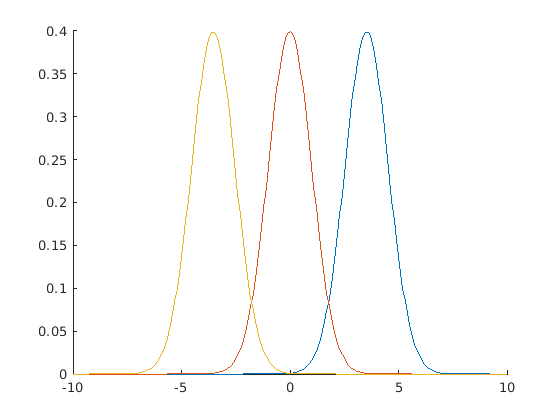
\includegraphics[scale=0.6]{3}

\subsection{Question 4}

\begin{verbatim}
  r=RxSignal(1,:);
  d=500;
  [h, x]=hist(r,d);
  lr=length(r);
  lh=x(end)-x(1)
  plot(x,h.*(d/(lr*lh)));
\end{verbatim}
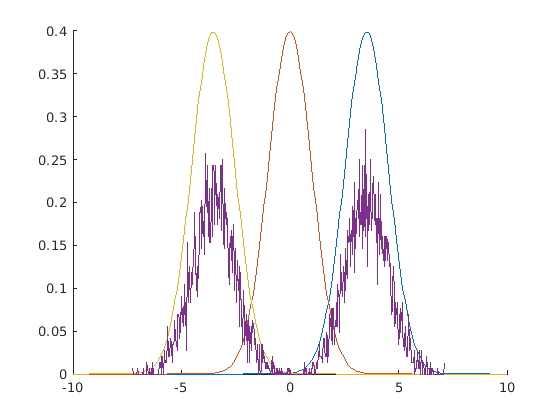
\includegraphics[scale=0.6]{4}

We can appreciate that the pdf that fits better our experimental data is the one associated with $\phi=\frac{3\pi}{4}$, which will be our estimation.

\subsection{Question 5}
We are taking samples in the space domain because we want all the samples to belong to the same pdf for easy matching. If we took the samples at different times each sample would have a different pdf associated with them and thus the method we applied here wouldn't work.

To be able to treat space and time indistictly as domains, the pdfs of the values at different times would need to be the same.
\subsection{Question 6}
Following the instructions:
\begin{verbatim}
  x=0:0.1:2*pi;
  y = (1/(sigma*sqrt(2*pi))).*exp(
    -((RxSignal(1,1)-5*cos(x)).^2)/(2*sigma^2));
  plot(x,y);
\end{verbatim}

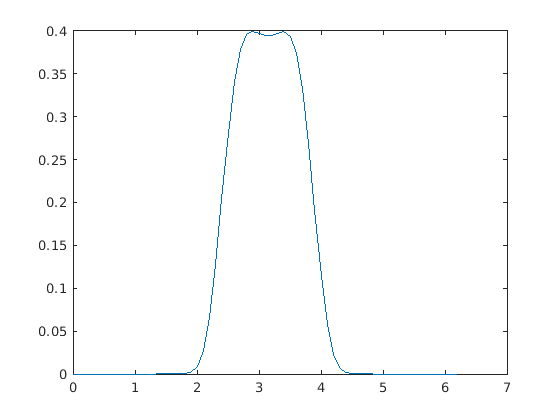
\includegraphics[scale=0.6]{6}

An explanation for why we are seeing two peaks on this graph can be found on the answer to question 7.

\subsection{Question 7}
We will estimate $\phi$ by finding the value on the x axis where the likelihood function has a maximum:
\begin{verbatim}
  find(y==max(y))
\end{verbatim}

The estimation from our single sample is $3.5$, but this estimation is prone to error since it uses a single sample. Note that we must consider that the value we are using in our likelihood function is $cos(\phi)$, so if the maximum is on 3.5 this would mean that $\phi$ is either $3.5$ or $3.5-2(3.5-\pi)$ as both of these values provide the same result when applied to $cos()$.

To provide a better estimation we could use all the samples on the same time-dimension (thus all the ones that share the same pdf) and calculate the ML estimate for each of them:

\begin{verbatim}
  x=0:0.1:2*pi;
  count=zeros(length(x));
  for i=1:length(RxSignal(1,:))
      y = (1/(sigma*sqrt(2*pi))).*exp(-((RxSignal(1,i)-5*cos(x)).^2)/(2*sigma^2));
      f=find(y==max(y));
      count(f)=count(f)+1;
  end
  plot(x, count)
\end{verbatim}

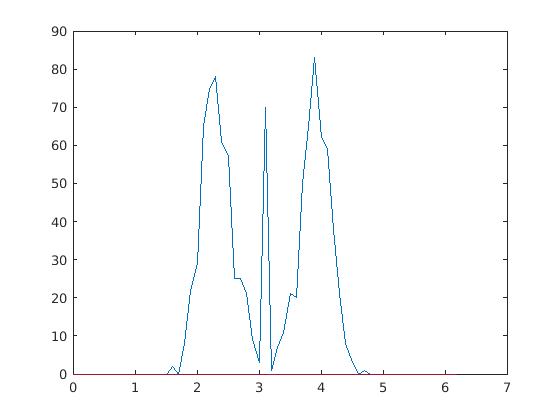
\includegraphics[scale=0.6]{all}

Here we see two peaks at $x=2.3\approx \frac{3\pi}{4}$ and $x=3.9 \approx \frac{5\pi}{4}$. These two match with the estimate $\phi=\frac{3\pi}{4}$ that we saw on question 4, as the value that we are using for our likelihood function is $cos(\phi)$ and $cos(\frac{3\pi}{4})=cos(\frac{5\pi}{4})$.

On top of that we can appreciate a peak at $x=3.1$ which I don't know how to explain as of now.

In any case, we can see that there are some estimations on $x=1.6$, which is really far away from the real value of $\phi$. This is the problem that estimations based on a single realization have, that if you use an atypical realization your estimate will end up skewed.

\section{Conclusion}
We managed to obtain a good estimate of the signal's phase, thus accomplishing our objectives.


\end{document}


